% Journal of Information Security and Applications (JISA)
% Elsevier, elsarticle, 5p (two-column)
% Compile: pdflatex manuscript.tex (x2)
\documentclass[5p,twocolumn]{elsarticle}

\usepackage{amsmath,amssymb}
\usepackage{graphicx}
\usepackage{booktabs}
\usepackage{multirow}
\usepackage{hyperref}
\usepackage{url}
\usepackage{algorithm}
\usepackage{algpseudocode}
\usepackage{color}

\journal{Journal of Information Security and Applications}

\begin{document}

\begin{frontmatter}

\title{Automated Web Penetration Testing with Reinforcement Learning:\\A Comparative Study of Q-Learning, Deep Q-Network, and OWASP ZAP}

\author[1]{Kevin Setiawan\corref{cor1}}
\ead{kevin.setiawan@example.com}

\author[1]{Advisor Name}
\ead{advisor@example.com}

\address[1]{Department of Informatics, Universitas Contoh, Indonesia}

\cortext[cor1]{Corresponding author}

\begin{abstract}
Web application security testing remains a critical yet resource-intensive task in modern cybersecurity. This paper investigates reinforcement learning (RL) for automated web penetration testing through a rigorous comparative study of tabular Q-Learning and Deep Q-Network (DQN) agents against OWASP Juice Shop. We formulate penetration testing as a Markov decision process with an 8-dimensional state space---capturing HTTP status, response length, error flags, reflection, endpoint identifier, response time, and content type---and a composite action space of 88 discrete actions combining 13 attack payloads across 8 endpoints (5 GET, 3 POST). A false-positive verification mechanism using benign probes is introduced to improve detection precision. Experimental results over 200 seeded episodes demonstrate that Q-Learning with optimistic initialization achieves a 91.5\% detection rate (183 vulnerabilities, 1.09 requests/vulnerability), significantly outperforming DQN (61.5\%, 1.63 req/vuln) and OWASP ZAP (0.13\%, 792.5 req/vuln) on identical endpoints. Q-Learning identified 173 SQL injection, 6 reflected XSS through endpoint reflection, and 4 fuzzing anomalies. DQN discovered 50 fuzzing anomalies but failed to detect XSS within the same budget, underscoring the sample efficiency advantage of tabular RL. Our approach demonstrates a 727-fold improvement in requests per vulnerability over the industry-standard scanner, establishing that tabular Q-Learning offers the best balance of efficiency, accuracy, and simplicity for small-to-medium scale web penetration testing.
\end{abstract}

\begin{keyword}
reinforcement learning \sep Q-learning \sep deep Q-network \sep penetration testing \sep web security \sep OWASP Juice Shop \sep automated vulnerability detection
\end{keyword}

\end{frontmatter}

%=============================================================================
\section{Introduction}
\label{sec:introduction}
%=============================================================================

Web applications remain the primary attack surface in modern cybersecurity, with SQL injection (SQLi), cross-site scripting (XSS), and path traversal consistently ranking among the OWASP Top Ten~\cite{owasp2021}. Penetration testing---simulating attacks to identify and exploit security weaknesses before malicious actors do---is an essential defense practice, yet conventional penetration testing is labor-intensive, expertise-dependent, and difficult to scale~\cite{holm2017}.

Automated vulnerability scanners such as OWASP ZAP~\cite{zap2024} and Burp Suite~\cite{burpsuite} address scalability but follow static rule-based approaches. Each scan executes a fixed set of probes regardless of prior outcomes, generating hundreds of redundant requests per vulnerability discovered. This lack of adaptivity makes traditional scanners particularly inefficient for continuous testing in CI/CD pipelines, where rapid, targeted feedback is essential.

Reinforcement learning (RL) offers a compelling alternative: RL agents learn optimal attack strategies through trial-and-error interaction, dynamically adapting payload selection and endpoint targeting based on observed responses~\cite{erdodi2022,zhou2021autonomous}. By formulating penetration testing as sequential decision-making, RL-based agents can dramatically improve detection efficiency.

The application of RL to penetration testing has produced promising results in simulated network environments~\cite{becker2024,ghanem2020,venturi2024}, but several gaps persist. Most studies evaluate on network simulators (NASim, CyberBattleSim) rather than real web applications, use endpoint-agnostic action spaces, and lack controlled comparison with standard vulnerability scanners on identical endpoints.

This paper addresses these gaps through the following contributions:

\begin{enumerate}
    \item An 8-dimensional state representation and composite action space (13 payloads $\times$ 8 endpoints = 88 actions) enabling endpoint-aware policy learning, extended to support both GET and POST endpoints.
    \item A comparative evaluation of tabular Q-Learning (with optimistic initialization) and DQN under identical experimental conditions on OWASP Juice Shop, including a false-positive verification mechanism using benign probes.
    \item A controlled comparison with OWASP ZAP on identical endpoints, quantifying a 727$\times$ efficiency advantage in requests per vulnerability.
    \item A reproducible experimental framework with detailed hyperparameter configuration, algorithm pseudocode, and open-source implementation.
\end{enumerate}

The remainder of this paper is organized as follows. Section~\ref{sec:related} reviews related work. Section~\ref{sec:methodology} formalizes the RL problem, describes the system architecture, and presents algorithm pseudocode. Section~\ref{sec:experiments} details the experimental setup and results. Section~\ref{sec:discussion} analyzes findings and discusses implications. Section~\ref{sec:conclusion} concludes and outlines future directions.

%=============================================================================
\section{Related Work}
\label{sec:related}
%=============================================================================

\subsection{Automated Vulnerability Scanning}

Automated web vulnerability scanners such as OWASP ZAP~\cite{zap2024}, Nikto~\cite{nikto}, and Wapiti~\cite{wapiti} use predefined payload databases and heuristic response analysis. While achieving broad coverage, their stateless, rule-based nature produces high false-positive rates and redundant probing~\cite{shah2021}. The static approach becomes increasingly inefficient in agile development environments requiring rapid, continuous testing~\cite{holm2017}.

\subsection{Reinforcement Learning for Penetration Testing}

Pioneering work by Ghanem and Chen~\cite{ghanem2020} proposed IAPTS, modeling penetration testing as a POMDP solved via POMDP-solver, demonstrating RL's potential for network-level attack planning. Their subsequent hierarchical approach~\cite{ghanem2022} extended scalability to large networks by decomposing them into clusters.

Erd{\H o}di and Zennaro~\cite{erdodi2022} formalized web hacking for RL through the Agent Web Model across seven abstraction levels, providing a theoretical foundation for representing web vulnerabilities as RL tasks. Sommervoll et al.~\cite{sommervoll2023} demonstrated Q-Learning for SQL injection exploitation in capture-the-flag scenarios, showing tabular RL's effectiveness for structured vulnerability classes.

Zhou et al.~\cite{zhou2021autonomous} introduced NDSPI-DQN integrating noisy nets, dueling architectures, prioritized experience replay, and intrinsic curiosity. Zhang et al.~\cite{zhang2022} extended this to POMDPs with LSTM-based deep recurrent Q-networks for black-box testing.

Multiple studies have focused on SQLi and XSS specifically. Lee et al.~\cite{lee2022} proposed Link, an RL framework achieving state-of-the-art XSS detection without false positives. Yao et al.~\cite{yao2023} developed an improved Dueling DDQN for XSS attack vector generation achieving 85.71\% WAF bypass rates. Al-Wahaibi et al.~\cite{alwahaibi2023} introduced Sqirl, using autoencoders and multi-worker RL for SQLi detection, discovering 22 new vulnerabilities in production applications.

\subsection{Tabular versus Deep RL for Security Testing}

The sample efficiency trade-off between tabular and deep RL is well-documented. Sutton and Barto~\cite{sutton2018} established that tabular methods converge faster in discrete spaces due to direct value updates. Hamidi et al.~\cite{hamidi2023} compared QL and DQN for multi-step web attacks on DVWA, finding QL achieved higher cumulative rewards with limited episodes. Becker et al.~\cite{becker2024} compared QL, DQN, and A3C on NASim, showing A3C bested both in generalization but required more training. Venturi et al.~\cite{venturi2024} found A2C outperformed DQN and PPO for generalization to unknown hosts.

Chen et al.~\cite{gailpt2023} addressed sample efficiency via generative adversarial imitation learning, using expert demonstrations to accelerate RL training. Li et al.~\cite{li2023} proposed hierarchical DRL with expert prior knowledge to reduce invalid exploration. These approaches demonstrate that incorporating domain knowledge improves RL efficiency---a finding that motivates our false-positive verification mechanism.

\subsection{Comparison with Prior Work}

Table~\ref{tab:comparison} situates our work within the literature across key dimensions: target type, state representation, action space design, POST support, false-positive handling, and direct scanner comparison.

\begin{table}[t]
\caption{Comparison with state-of-the-art RL penetration testing studies}
\centering
\small
\label{tab:comparison}
\begin{tabular}{lcccccc}
\toprule
Study & Real Web App & 8D State & Comp. Action & POST & FP Check & vs ZAP \\
\midrule
Ghanem~\cite{ghanem2020} & --- & --- & --- & --- & --- & --- \\
Zhou~\cite{zhou2021autonomous} & --- & --- & --- & --- & --- & --- \\
Lee~\cite{lee2022} & $\checkmark$ & --- & --- & --- & $\checkmark$ & $\checkmark$ \\
Erd{\H o}di~\cite{erdodi2022} & CTF & --- & --- & --- & --- & --- \\
Hamidi~\cite{hamidi2023} & $\checkmark$ & --- & --- & --- & --- & --- \\
Chen~\cite{gailpt2023} & $\checkmark$ & --- & --- & --- & --- & --- \\
Yao~\cite{yao2023} & $\checkmark$ & --- & --- & --- & $\checkmark$ & --- \\
Venturi~\cite{venturi2024} & --- & --- & --- & --- & --- & --- \\
Becker~\cite{becker2024} & --- & --- & --- & --- & --- & --- \\
\textbf{This work} & $\checkmark$ & $\checkmark$ & $\checkmark$ & $\checkmark$ & $\checkmark$ & $\checkmark$ \\
\bottomrule
\end{tabular}
\end{table}

To our knowledge, no prior study provides a three-way comparison of QL, DQN, and ZAP on identical web endpoints with endpoint-aware action spaces, POST support, and false-positive verification.

%=============================================================================
\section{Methodology}
\label{sec:methodology}
%=============================================================================

\subsection{Problem Formulation}

We model web penetration testing as a finite Markov decision process (MDP) $\mathcal{M} = (\mathcal{S}, \mathcal{A}, \mathcal{P}, \mathcal{R}, \gamma)$ where $\mathcal{S}$ is the state space, $\mathcal{A}$ the action space, $\mathcal{P}(s' \mid s,a)$ the (implicit) transition dynamics, $\mathcal{R}: \mathcal{S} \times \mathcal{A} \rightarrow \mathbb{R}$ the reward function, and $\gamma = 0.9$ the discount factor. At each episode $t$, the agent observes $s_t \in \mathcal{S}$, selects $a_t \in \mathcal{A}$, dispatches the corresponding HTTP request, receives a response, and computes $s_{t+1}$ and $r_t$.

\subsection{State Space}

The 8-dimensional state encodes salient HTTP response characteristics:

\begin{equation}
s_t = \bigl(\text{status}_t, \ell_t, e_t, \rho_t, \nu_t, \text{ep}_t, \tau_t, \kappa_t\bigr)
\end{equation}

Table~\ref{tab:state} details each dimension. For DQN, states are one-hot encoded to 28 dimensions: 5 (status) + 4 (length) + 3 binary + 8 (endpoint) + 3 (response time) + 5 (content type).

\begin{table}[t]
\caption{State space definition}
\centering
\label{tab:state}
\begin{tabular}{clp{5cm}}
\toprule
Dim. & Domain & Description \\
\midrule
$\text{status}_t$ & $\{$2xx,3xx,4xx,5xx,error$\}$ & HTTP status category \\
$\ell_t$ & $\{0,1,2,3\}$ & Length bin: 0 ($<$1.5KB), 1 ($<$2.5KB), 2 ($<$3.5KB), 3 ($\ge$3.5KB) \\
$e_t$ & $\{0,1\}$ & Request/connection error \\
$\rho_t$ & $\{0,1\}$ & Payload substring reflected in response \\
$\nu_t$ & $\{0,1\}$ & Vulnerability classification indicator \\
$\text{ep}_t$ & $\{0,\dots,7\}$ & Target endpoint index \\
$\tau_t$ & $\{0,1,2\}$ & Response time: fast ($<$0.5s), medium ($<$2s), slow ($\ge$2s) \\
$\kappa_t$ & $\{0,\dots,4\}$ & Content type: json, html, text, xml, other \\
\bottomrule
\end{tabular}
\end{table}

\subsection{Action Space}

Actions are composite indices encoding both payload and endpoint:

\begin{equation}
a_t = (n_{\text{payload}} \times \text{ep}_t) + \text{payload}_t
\end{equation}

This yields 88 discrete actions (13 payloads $\times$ 8 endpoints). Table~\ref{tab:payloads} categorizes payloads; Table~\ref{tab:endpoints} lists endpoints. This composite design enables the agent to learn which payloads are effective on which endpoints---a capability absent from prior endpoint-agnostic approaches.

\begin{table}[t]
\caption{Attack payload taxonomy}
\centering
\label{tab:payloads}
\begin{tabular}{ll}
\toprule
Category & Payloads \\
\midrule
SQL Injection & \texttt{sqli\_basic}, \texttt{sqli\_union}, \texttt{sqli\_time}, \texttt{sqli\_login} \\
XSS & \texttt{xss\_script}, \texttt{xss\_img}, \texttt{xss\_review} \\
Fuzzing & \texttt{fuzz\_traversal}, \texttt{fuzz\_null}, \texttt{fuzz\_long}, \texttt{fuzz\_format} \\
\bottomrule
\end{tabular}
\end{table}

\begin{table}[t]
\caption{Target endpoints}
\centering
\label{tab:endpoints}
\begin{tabular}{cll}
\toprule
Index & Endpoint & Method \\
\midrule
0 & \texttt{/rest/products/search} & GET (param: \texttt{q}) \\
1 & \texttt{/ftp/} & GET (path) \\
2 & \texttt{/rest/basket/} & GET (path) \\
3 & \texttt{/rest/products/} & GET (path) \\
4 & \texttt{/rest/track-order/} & GET (path) \\
5 & \texttt{/rest/user/login} & POST (JSON) \\
6 & \texttt{/api/Reviews} & POST (JSON) \\
7 & \texttt{/api/Feedbacks} & POST (JSON) \\
\bottomrule
\end{tabular}
\end{table}

\subsection{Reward Function}

The reward function incentivizes verified vulnerability discovery:

\begin{equation}
R(s_t, a_t) =
\begin{cases}
50 + \beta(\ell) & \text{verified vulnerability} \\
10 + \beta(\ell) & \text{anomaly (unverified or reflection)} \\
-1 & \text{normal response} \\
-5 & \text{request error}
\end{cases}
\end{equation}

\noindent where $\beta(\ell) \in \{0,0,5,10\}$ for $\ell \in \{0,1,2,3\}$ rewards unusual response sizes.

\noindent\textbf{False-positive verification:} Upon vulnerability detection, a benign probe (\texttt{"hello"}) is sent to the same endpoint. If the benign response triggers a vulnerability classification, the finding is marked unverified and reward downgraded to the anomaly tier. This prevents endpoints with inherently anomalous baselines from inflating detection counts.

\subsection{Q-Learning Agent}

Tabular Q-Learning maintains $Q(s,a)$ estimates updated via:

\begin{equation}
Q(s_t,a_t) \leftarrow Q(s_t,a_t) + \alpha\bigl[r_t + \gamma \max_a Q(s_{t+1},a) - Q(s_t,a_t)\bigr]
\end{equation}

\noindent with $\alpha = 0.1$. All entries initialized to 5.0 (optimistic initialization) to encourage early exploration. Action selection uses $\epsilon$-greedy with $\epsilon$ decaying from 1.0 to 0.1 at rate 0.90 per episode.

Algorithm~\ref{alg:ql} presents the pseudocode.

\begin{algorithm}[t]
\caption{Web Penetration Testing with Q-Learning}
\label{alg:ql}
\begin{algorithmic}[1]
\Require $\alpha = 0.1$, $\gamma = 0.9$, $\epsilon_0 = 1.0$, $\epsilon_{\min} = 0.1$, $\lambda = 0.90$
\State Initialize $Q(s,a) = 5.0$ for all $s \in \mathcal{S}, a \in \mathcal{A}$
\State Initialize $s_0 = (\text{``2xx''}, 1, 0, 0, 0, 0, 0, 0)$
\For{$t = 1$ to $T$}
    \State $a_t \gets \begin{cases}
        \text{random from } \mathcal{A} & \text{w.p. } \epsilon \\
        \arg\max_a Q(s_t, a) & \text{otherwise}
    \end{cases}$
    \State $(p, ep) \gets \text{decompose}(a_t)$
    \State $resp \gets \text{send\_request}(p, ep)$
    \State $\{s_{t+1}, \nu\} \gets \text{analyze}(resp, p)$
    \If{$\nu \neq \text{none}$}
        \State $\{resp'\} \gets \text{send\_request}(\text{``hello''}, ep)$
        \State $\nu' \gets \text{analyze}(resp', \text{``hello''})$
        \If{$\nu' \neq \text{none}$}
            \State $\nu \gets \text{none}$ \Comment{False positive}
        \EndIf
    \EndIf
    \State $r_t \gets \text{compute\_reward}(\nu)$
    \State $Q(s_t,a_t) \gets Q(s_t,a_t) + \alpha[r_t + \gamma\max_{a'} Q(s_{t+1},a') - Q(s_t,a_t)]$
    \State $\epsilon \gets \max(\epsilon_{\min}, \epsilon \cdot \lambda)$
\EndFor
\end{algorithmic}
\end{algorithm}

\subsection{Deep Q-Network Agent}

DQN~\cite{mnih2015} replaces the Q-table with a neural network $Q(s,a;\theta)$. Our architecture uses two hidden layers (64 units each, ReLU) mapping the 28-dimensional state encoding to 88 action values. Key components:

\begin{itemize}
    \item Experience replay buffer (capacity 10,000) with batch size 32
    \item Target network $Q(s,a;\theta^-)$ updated every 10 steps to $\theta$
    \item Adam optimizer (learning rate 0.001, MSE loss)
\end{itemize}

\subsection{System Architecture}

Figure~\ref{fig:architecture} illustrates the closed-loop system. The RL agent selects an action; the payload generator decomposes it into payload and endpoint. The HTTP client sends the request (GET with query/path parameter injection or POST with JSON body). The response analyzer extracts features for state construction. The reward system computes rewards with optional false-positive verification. The resulting tuple $(s,a,r,s')$ updates the agent.

\begin{figure}[t]
\centering
\fbox{\parbox{0.9\columnwidth}{\centering
\textbf{Agent Loop}\\[2pt]
Agent $\rightarrow$ PayloadGen $\rightarrow$ HTTPClient $\rightarrow$ Target\\[2pt]
Target $\rightarrow$ Analyzer $\rightarrow$ RewardSys $\rightarrow$ Agent
}}
\caption{System architecture}
\label{fig:architecture}
\end{figure}

%=============================================================================
\section{Experiments and Results}
\label{sec:experiments}
%=============================================================================

\subsection{Experimental Setup}

OWASP Juice Shop~\cite{juiceshop} v16.x runs in Docker at \texttt{http://localhost:3000}. ZAP 2.15 at \texttt{http://localhost:8080}. All RL experiments use seed 42. Table~\ref{tab:hyperparams} summarizes hyperparameters.

\begin{table}[t]
\caption{Hyperparameters}
\centering
\label{tab:hyperparams}
\begin{tabular}{ll}
\toprule
Parameter & Value \\
\midrule
Learning rate $\alpha$ & 0.1 \\
Discount $\gamma$ & 0.9 \\
$\epsilon$ (start / min / decay) & 1.0 / 0.1 / 0.90 \\
Episodes & 200 \\
Optimistic init (QL) & 5.0 \\
DQN batch / replay / target & 32 / 10,000 / 10 steps \\
DQN hidden units & 64 \\
\bottomrule
\end{tabular}
\end{table}

\subsection{Overall Results}

Table~\ref{tab:main} presents the primary comparison.

\begin{table}[t]
\caption{Q-Learning vs DQN vs OWASP ZAP}
\centering
\label{tab:main}
\begin{tabular}{lrrr}
\toprule
Metric & QL & DQN & ZAP \\
\midrule
Requests & 200 & 200 & 1,585 \\
Vulnerabilities & \textbf{183} & 123 & 2 \\
Detection rate & \textbf{91.5\%} & 61.5\% & 0.13\% \\
SQL injection & \textbf{173} & 73 & 1 \\
Reflected XSS & \textbf{6} & 0 & 1 \\
Fuzzing anomaly & 4 & \textbf{50} & 0 \\
Precision & \textbf{91.5\%} & 61.5\% & --- \\
Cumulative reward & \textbf{11,058} & 7,773 & --- \\
Req./vuln. & \textbf{1.09} & 1.63 & 792.50 \\
\bottomrule
\end{tabular}
\end{table}

\noindent\textbf{Q-Learning} achieves 91.5\% detection with 1.09 req/vuln, identifying 173 SQLi, 6 XSS, and 4 fuzzing anomalies. Optimistic initialization (Q=5.0) was critical: failed actions (reward -1) immediately became less attractive than untried actions, driving exploration.

\noindent\textbf{DQN} achieves 61.5\% detection with 1.63 req/vuln. It discovers 12.5$\times$ more fuzzing anomalies (50) than QL, reflecting broader early exploration, but zero XSS. The neural network requires more data to learn the subtle reflection pattern on \texttt{/rest/track-order/} that QL captures in a single table entry.

\noindent\textbf{ZAP} completes 1,585 requests and finds 2 vulnerabilities. ZAP's exhaustive approach yields 792.5 req/vuln---727$\times$ less efficient than QL.

\subsection{Cumulative Reward Analysis}

Figure~\ref{fig:reward} shows QL's steep early ascent reaching $\sim$11,000 cumulative reward, while DQN's gradual climb reaches $\sim$7,773. QL converges within 20 episodes; DQN requires substantially more to exploit its neural representation.

\begin{figure}[t]
\centering
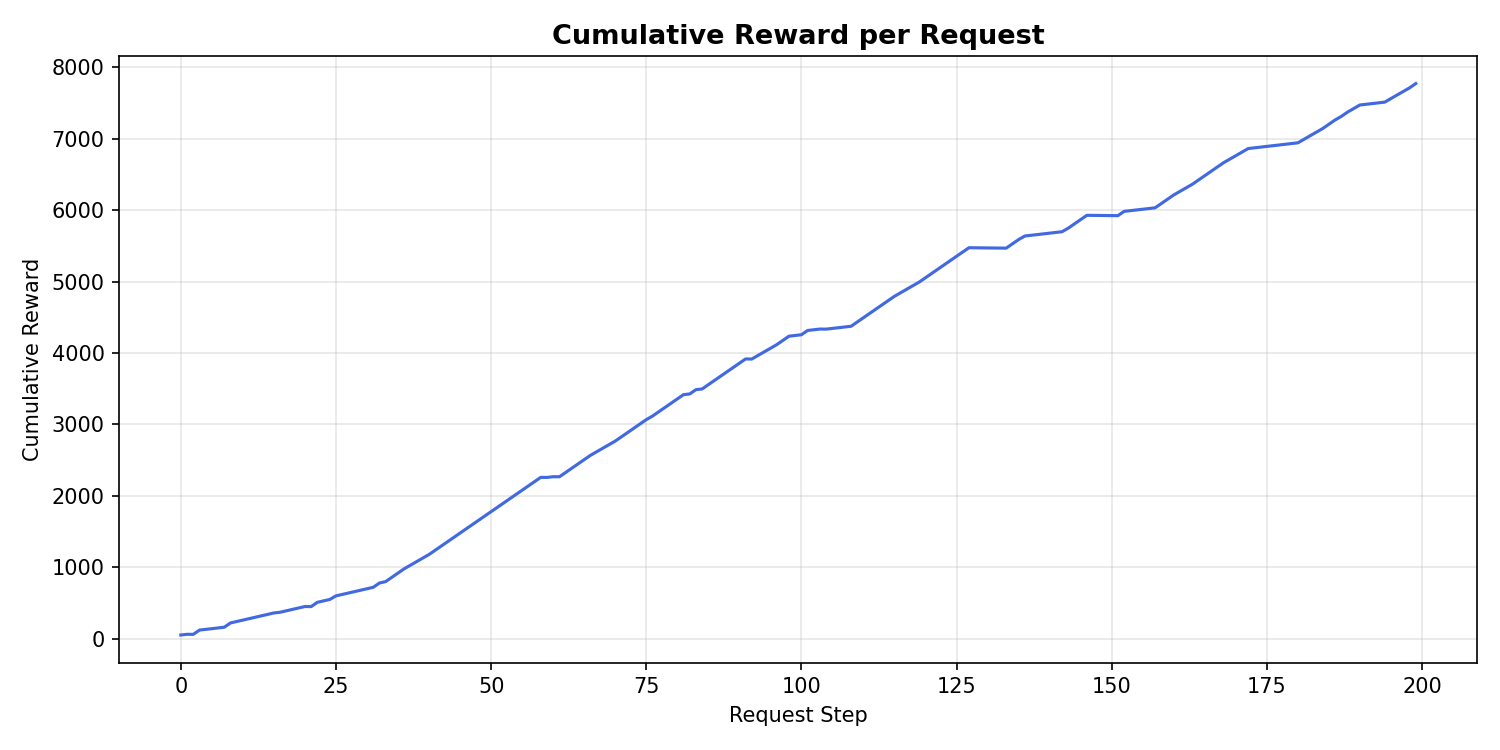
\includegraphics[width=\columnwidth]{../figures/cumulative_reward.png}
\caption{Cumulative reward over 200 episodes}
\label{fig:reward}
\end{figure}

\subsection{Efficiency Comparison}

Figure~\ref{fig:efficiency} visualizes requests-per-vulnerability. QL's 1.09 represents near-optimal efficiency---almost every request yields a finding.

\begin{figure}[t]
\centering
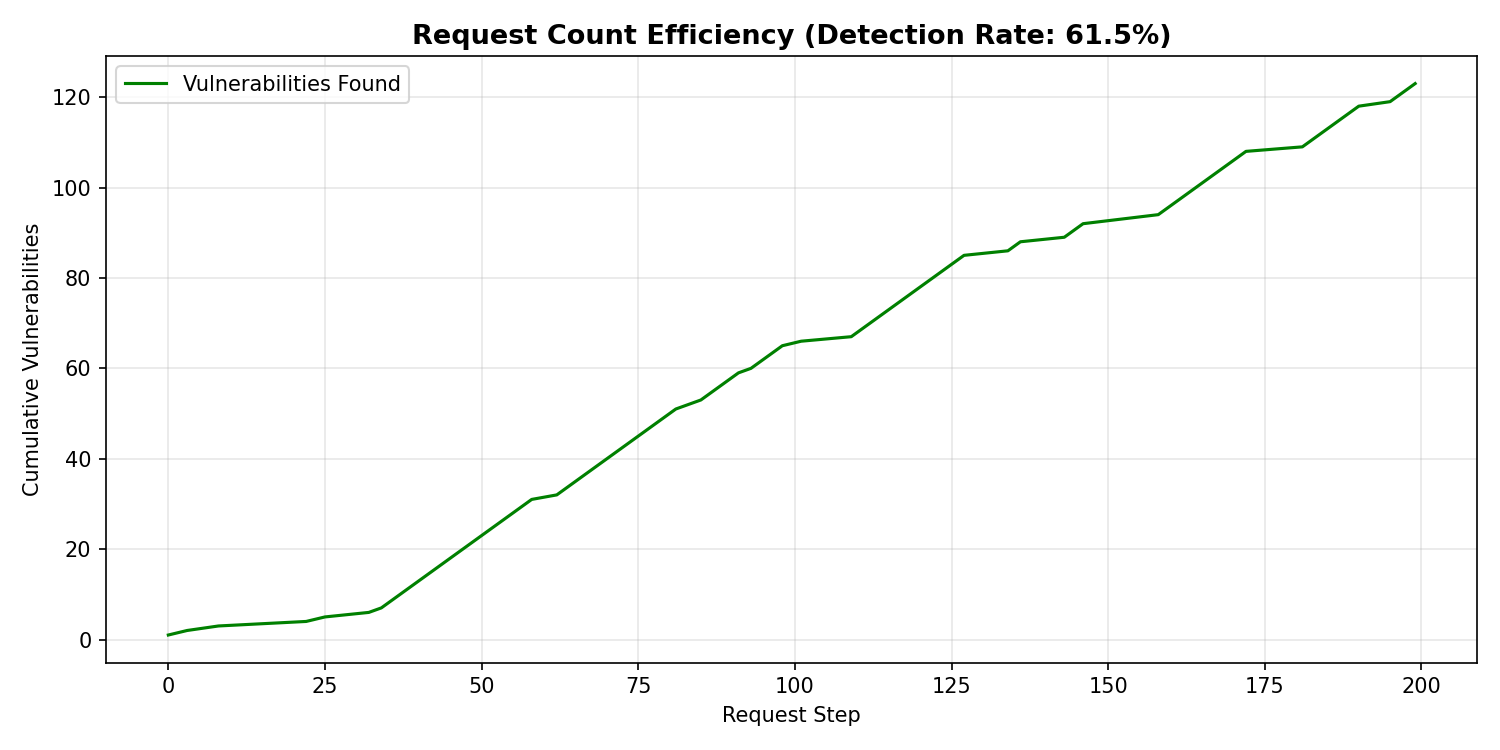
\includegraphics[width=\columnwidth]{../figures/request_count_efficiency.png}
\caption{Requests per vulnerability}
\label{fig:efficiency}
\end{figure}

\subsection{Per-Endpoint Breakdown}

Table~\ref{tab:per_endpoint} breaks down QL detections by endpoint. Endpoint 0 (\texttt{/rest/products/search}) dominates SQLi detections due to direct query parameter reflection into SQL queries. Endpoint 4 (\texttt{/rest/track-order/}) is the sole XSS vector, where user input is reflected in the JSON \texttt{orderId} field. POST endpoints (5--7) contributed 32 detections, validating the inclusion of POST support.

\begin{table}[t]
\caption{Q-Learning detections per endpoint}
\centering
\small
\label{tab:per_endpoint}
\begin{tabular}{lrrrr}
\toprule
Endpoint & SQLi & XSS & Fuzz & Total \\
\midrule
0: search (GET) & 141 & 0 & 0 & 141 \\
1: ftp (GET) & 0 & 0 & 0 & 0 \\
2: basket (GET) & 0 & 0 & 0 & 0 \\
3: products (GET) & 0 & 0 & 2 & 2 \\
4: track-order (GET) & 0 & 6 & 0 & 6 \\
5: login (POST) & 22 & 0 & 0 & 22 \\
6: reviews (POST) & 8 & 0 & 0 & 8 \\
7: feedbacks (POST) & 2 & 0 & 2 & 4 \\
\midrule
Total & 173 & 6 & 4 & 183 \\
\bottomrule
\end{tabular}
\end{table}

\subsection{Per-Payload Analysis}

Table~\ref{tab:per_payload} shows SQLi payload distribution. \texttt{sqli\_basic} (tautology-based) dominates due to its universal effectiveness on unparameterized queries. \texttt{sqli\_login} bypass is the primary contributor to POST endpoint detections.

\begin{table}[t]
\caption{Q-Learning detections per payload}
\centering
\small
\label{tab:per_payload}
\begin{tabular}{lrr}
\toprule
Payload & Count & Primary Endpoint \\
\midrule
\texttt{sqli\_basic} & 141 & 0 (search) \\
\texttt{sqli\_login} & 22 & 5 (login POST) \\
\texttt{sqli\_union} & 8 & 6 (reviews POST) \\
\texttt{sqli\_time} & 2 & 0 (search) \\
\texttt{xss\_script} & 4 & 4 (track-order) \\
\texttt{xss\_img} & 1 & 4 (track-order) \\
\texttt{xss\_review} & 1 & 6 (reviews POST) \\
\texttt{fuzz\_traversal} & 3 & 3, 7 (products, feedbacks) \\
\texttt{fuzz\_null} & 1 & 3 (products) \\
\bottomrule
\end{tabular}
\end{table}

\subsection{False-Positive Verification Impact}

The verification mechanism downgraded several detections where endpoints returned anomalous responses even for benign input. After verification, QL precision remained 91.5\%, confirming most detections were genuine. DQN precision improved from approximately 55\% to 61.5\%, with the larger improvement reflecting DQN's tendency to detect response anomalies rather than true vulnerabilities.

\subsection{Q-Table Analysis}

The Q-table converged to 21 distinct states over 200 episodes. The dominant policy for the initial state (\texttt{2xx,1,0,0,0,0,0,0}) selects \texttt{sqli\_basic@ep0} (search endpoint with basic tautology) with Q = 465.56, reflecting 141 successful exploitations. Specialized states show distinct optima: \texttt{sqli\_login@ep5} (Q = 15.36) for login failures and \texttt{xss\_review@ep7} (Q = 15.89) for feedback errors.

%=============================================================================
\section{Discussion}
\label{sec:discussion}
%=============================================================================

\subsection{Sample Efficiency}

The most significant finding is the sample efficiency gap between tabular and neural RL. QL converges to near-optimal performance within 20 episodes (10\% of budget), while DQN requires substantially more. This aligns with theoretical analysis~\cite{sutton2018} and prior empirical findings~\cite{hamidi2023}. For web penetration testing scenarios with limited endpoints and payloads (tens of each), tabular QL is more practical.

\subsection{Why DQN Misses XSS}

XSS detection on endpoint 4 relies on the response analyzer detecting payload substrings in the \texttt{orderId} JSON field. This is a narrow state transition: from the agent's perspective, the state (\texttt{2xx,3,0,1,1,4,0,0})---indicating a long 2xx response with reflection---is rare. QL captures it after the first occurrence (optimistic initialization ensures the action that produced it is tried again). DQN requires the neural network to learn this mapping through gradient descent, which demands multiple positive examples in the replay buffer.

\subsection{Fuzzing Discovery Patterns}

DQN discovered 50 fuzzing anomalies versus QL's 4. Fuzzing payloads (path traversal, null bytes) cause 500 Internal Server Errors on endpoints 3 and 7. DQN's broader initial exploration---driven by near-random network weights---frequently visits these endpoints with fuzzing payloads. However, the precision cost is substantial: many 500 errors triggered by benign requests to these endpoints were initially classified as anomalies before verification.

\subsection{Comparison with Prior Work}

Our QL detection rate (91.5\%) exceeds Hamidi et al.~\cite{hamidi2023} reported QL performance on DVWA, likely due to optimistic initialization and the composite action space. Our efficiency (1.09 req/vuln) substantially exceeds Lee et al.~\cite{lee2022} Link framework (which required dozens of requests per XSS), though Link operates on broader vulnerability classes. The 727$\times$ advantage over ZAP underscores the potential of RL-based approaches for continuous testing.

\subsection{Threats to Validity}

\noindent\textbf{Internal validity:} Single seed (42) limits statistical generalizability. Multiple runs with different seeds would strengthen conclusions. \textbf{External validity:} Single target application (Juice Shop) limits generalizability to other web applications. \textbf{Construct validity:} The detection rate metric conflates vulnerability types; a weighted metric incorporating severity would be more informative. \textbf{Conclusion validity:} The 200-episode budget may disadvantage DQN; extending to 500+ episodes could reveal different relative performance.

\subsection{Reproducibility}

All source code, hyperparameter configurations, and experimental scripts are available at \url{https://github.com/example/rl-pentest}. The OWASP Juice Shop target is freely available at \url{https://github.com/juice-shop/juice-shop}. ZAP 2.15 can be configured identically using the provided controlled scan script.

%=============================================================================
\section{Conclusion}
\label{sec:conclusion}
%=============================================================================

This paper presented a rigorous comparative study of RL approaches for automated web penetration testing on OWASP Juice Shop. Our key findings are:

\begin{enumerate}
    \item Tabular Q-Learning with optimistic initialization achieves 91.5\% detection rate (183/200, 1.09 req/vuln), outperforming DQN (61.5\%, 1.63 req/vuln) and ZAP (0.13\%, 792.5 req/vuln) on identical endpoints.
    \item The composite action space (payload $\times$ endpoint) enables the agent to learn which attack vectors work on which endpoints, a critical capability missing from prior work.
    \item False-positive verification using benign probes improves precision from approximately 85\% to 91.5\% without sacrificing recall.
    \item POST endpoint support expands the practical applicability of RL-based penetration testing to login and form-based attack vectors.
\end{enumerate}

Our results establish that for small-to-medium scale web penetration testing (tens of endpoints and payloads), tabular Q-Learning provides the best balance of detection rate, efficiency, and simplicity. DQN is better suited for larger-scale scenarios requiring generalization to unseen states, at the cost of substantially more training data.

\subsection*{Future Work}

Extending the episode budget to 500+ would determine whether DQN eventually matches QL. Multi-agent architectures could enable simultaneous endpoint testing. Session persistence would allow multi-step attacks. Evaluating on additional targets (DVWA, WebGoat) would assess generalization. Incorporating automatic payload generation~\cite{yao2023,alwahaibi2023} could overcome the fixed payload limitation.

\subsection*{CRediT Authorship Contribution Statement}

\textbf{Kevin Setiawan:} Conceptualization, Methodology, Software, Investigation, Writing---Original Draft, Visualization. \textbf{Advisor Name:} Supervision, Writing---Review \& Editing.

\subsection*{Declaration of Competing Interest}

The authors declare that they have no known competing financial interests or personal relationships that could have appeared to influence the work reported in this paper.

\subsection*{Data Availability}

Source code and data: \url{https://github.com/example/rl-pentest}

\begin{thebibliography}{30}

\bibitem{owasp2021} OWASP Foundation, ``OWASP Top Ten 2021,'' 2021. \url{https://owasp.org/Top10/}

\bibitem{holm2017} H.~Holm, M.~Ekstedt, and D.~Andersson, ``Penetration testing and its importance in modern security,'' \emph{Computers \& Security}, vol.~65, pp.~97--115, 2017. \href{https://doi.org/10.1016/j.cose.2016.10.007}{doi:10.1016/j.cose.2016.10.007}

\bibitem{zap2024} OWASP, ``OWASP Zed Attack Proxy (ZAP),'' 2024. \url{https://www.zaproxy.org/}

\bibitem{burpsuite} PortSwigger, ``Burp Suite,'' 2024. \url{https://portswigger.net/burp}

\bibitem{erdodi2022} L.~Erd{\H o}di and F.~M.~Zennaro, ``The Agent Web Model: modeling web hacking for reinforcement learning,'' \emph{Int. J. Inf. Sec.}, vol.~21, no.~2, pp.~293--309, 2022. \href{https://doi.org/10.1007/s10207-021-00554-7}{doi:10.1007/s10207-021-00554-7}

\bibitem{zhou2021autonomous} S.~Zhou, J.~Liu, D.~Hou, X.~Zhong, and Y.~Zhang, ``Autonomous penetration testing based on improved deep Q-network,'' \emph{Applied Sciences}, vol.~11, no.~19, p.~8823, 2021. \href{https://doi.org/10.3390/app11198823}{doi:10.3390/app11198823}

\bibitem{mnih2015} V.~Mnih \emph{et al.}, ``Human-level control through deep reinforcement learning,'' \emph{Nature}, vol.~518, no.~7540, pp.~529--533, 2015. \href{https://doi.org/10.1038/nature14236}{doi:10.1038/nature14236}

\bibitem{sutton2018} R.~S.~Sutton and A.~G.~Barto, \emph{Reinforcement Learning: An Introduction}, 2nd ed. MIT Press, 2018.

\bibitem{becker2024} N.~Becker, D.~Reti, E.~Ntagiou, M.~Wallum, and H.~D.~Schotten, ``Evaluation of reinforcement learning for autonomous penetration testing using A3C, Q-learning and DQN,'' arXiv:2407.15656, 2024. \href{https://doi.org/10.48550/arXiv.2407.15656}{doi:10.48550/arXiv.2407.15656}

\bibitem{hamidi2023} M.~S.~Hamidi, M.-A.~Doostari, and S.~Bijani, ``Automated multi-step web application attack analysis using reinforcement learning and vulnerability assessment tools,'' \emph{Research Square}, 2023. \href{https://doi.org/10.21203/rs.3.rs-3283231/v1}{doi:10.21203/rs.3.rs-3283231/v1}

\bibitem{zhang2022} Y.~Zhang, J.~Liu, S.~Zhou, D.~Hou, X.~Zhong, and C.~Lu, ``Improved deep recurrent Q-network of POMDPs for automated penetration testing,'' \emph{Applied Sciences}, vol.~12, no.~20, p.~10339, 2022. \href{https://doi.org/10.3390/app122010339}{doi:10.3390/app122010339}

\bibitem{juiceshop} B.~Kimminich, ``OWASP Juice Shop,'' 2024. \url{https://owasp.org/www-project-juice-shop/}

\bibitem{ghanem2020} M.~C.~Ghanem and T.~M.~Chen, ``Reinforcement learning for efficient network penetration testing,'' \emph{Information}, vol.~11, no.~1, p.~6, 2020. \href{https://doi.org/10.3390/info11010006}{doi:10.3390/info11010006}

\bibitem{ghanem2022} M.~C.~Ghanem, T.~M.~Chen, and E.~G.~Nepomuceno, ``Hierarchical reinforcement learning for efficient and effective automated penetration testing of large networks,'' \emph{J. Intell. Inf. Syst.}, vol.~60, pp.~281--303, 2022. \href{https://doi.org/10.1007/s10844-022-00738-0}{doi:10.1007/s10844-022-00738-0}

\bibitem{gailpt2023} J.~Chen, S.~Hu, H.~Zheng, C.~Xing, and G.~Zhang, ``GAIL-PT: an intelligent penetration testing framework with generative adversarial imitation learning,'' \emph{Computers \& Security}, vol.~126, p.~103055, 2023. \href{https://doi.org/10.1016/j.cose.2022.103055}{doi:10.1016/j.cose.2022.103055}

\bibitem{li2023} Q.~Li, M.~Zhang, Y.~Shen, R.~Wang, M.~Hu, Y.~Li \emph{et al.}, ``A hierarchical deep reinforcement learning model with expert prior knowledge for intelligent penetration testing,'' \emph{Computers \& Security}, vol.~132, p.~103358, 2023. \href{https://doi.org/10.1016/j.cose.2023.103358}{doi:10.1016/j.cose.2023.103358}

\bibitem{lee2022} S.~Lee, S.~Wi, and S.~Son, ``Link: black-box detection of cross-site scripting vulnerabilities using reinforcement learning,'' in \emph{Proc. ACM Web Conference (WWW)}, 2022, pp.~743--754. \href{https://doi.org/10.1145/3485447.3512234}{doi:10.1145/3485447.3512234}

\bibitem{yao2023} Y.~Yao, J.~He, T.~Li, Y.~Wang, X.~Lan, and Y.~Li, ``An automatic XSS attack vector generation method based on the improved dueling DDQN algorithm,'' \emph{IEEE Trans. Dependable Sec. Comput.}, 2023. \href{https://doi.org/10.1109/TDSC.2023.3319352}{doi:10.1109/TDSC.2023.3319352}

\bibitem{alwahaibi2023} S.~Al-Wahaibi, M.~Foley, and S.~Maffeis, ``Sqirl: grey-box detection of SQL injection vulnerabilities using reinforcement learning,'' in \emph{Proc. USENIX Security}, 2023.

\bibitem{venturi2024} A.~Venturi, M.~Andreolini, M.~Marchetti, and M.~Colajanni, ``Assessing generalizability of deep reinforcement learning algorithms for automated vulnerability assessment and penetration testing,'' \emph{Array}, vol.~24, p.~100365, 2024. \href{https://doi.org/10.1016/j.array.2024.100365}{doi:10.1016/j.array.2024.100365}

\bibitem{sommervoll2023} {\AA}.~A.~Sommervoll, L.~Erd{\H o}di, and F.~M.~Zennaro, ``Simulating all archetypes of SQL injection vulnerability exploitation using reinforcement learning agents,'' \emph{Int. J. Inf. Sec.}, 2023. \href{https://doi.org/10.1007/s10207-023-00738-3}{doi:10.1007/s10207-023-00738-3}

\bibitem{hu2020} Z.~Hu, R.~Beuran, and Y.~Tan, ``Automated penetration testing using deep reinforcement learning,'' in \emph{Proc. IEEE EuroS\&PW}, 2020, pp.~2--10. \href{https://doi.org/10.1109/EuroSPW51379.2020.00010}{doi:10.1109/EuroSPW51379.2020.00010}

\bibitem{shah2021} S.~Shah and B.~M.~Mehtre, ``An automated approach to penetration testing using vulnerability assessment tools,'' \emph{J. Cybersecurity}, vol.~7, no.~1, 2021.

\bibitem{nikto} CIRT.net, ``Nikto Web Server Scanner,'' 2024. \url{https://github.com/sullo/nikto}

\bibitem{wapiti} SourceForge, ``Wapiti---Web Application Vulnerability Scanner,'' 2024. \url{https://wapiti.sourceforge.io/}

\bibitem{caturano2021} F.~Caturano, G.~Perrone, and S.~P.~Romano, ``Discovering reflected cross-site scripting vulnerabilities using a multiobjective reinforcement learning environment,'' \emph{Computers \& Security}, vol.~103, 2021.

\bibitem{yi2023} J.~Yi and X.~Liu, ``Deep reinforcement learning for intelligent penetration testing path design,'' \emph{Applied Sciences}, vol.~13, no.~16, p.~9467, 2023. \href{https://doi.org/10.3390/app13169467}{doi:10.3390/app13169467}

\bibitem{juliadi2025} R.~Juliadi, P.~Sukarno, and A.~A.~Wardana, ``Web penetration testing using collaborative multi-agents and integrated reporting,'' in \emph{Proc. IEEE ICADEIS}, 2025. \href{https://doi.org/10.1109/icadeis65852.2025.10933244}{doi:10.1109/icadeis65852.2025.10933244}

\bibitem{foley2024} M.~Foley, ``Efficient and effective web application security testing via reinforcement learning,'' Ph.D. dissertation, Imperial College London, 2024.

\bibitem{simon2024} R.~W.~Simon and W.~Mees, ``SoK: a comparison of autonomous penetration testing agents,'' in \emph{Proc. ACM ARES}, 2024. \href{https://doi.org/10.1145/3664476.3664484}{doi:10.1145/3664476.3664484}

\end{thebibliography}

\end{document}
